\documentclass[11pt,a4paper]{article}

% Packages
\usepackage{geometry}
\usepackage{setspace}
\usepackage{graphicx}
\usepackage{lipsum}
\usepackage{url}
\usepackage{hyperref}
\usepackage{csquotes}
\usepackage{xcolor}
\usepackage{booktabs}

% Page formatting
\geometry{a4paper, margin=1in}
\renewcommand{\baselinestretch}{1.0}
\setlength{\parskip}{1em}
\pagenumbering{arabic}

% Bibliography
\usepackage[
    backend=biber,
    style=nature
]{biblatex}
\addbibresource{references.bib}

\begin{document}

% Title
\title{AI-assisted Design of virus-binding proteins for the International Genetically Engineered Machine comptetion}
\author{Tony MAKDISSY\thanks{Learning Planet Institute} \and 
Amir PANDI\thanks{Affiliation and role} \and 
Ariel LINDNER\thanks{Affiliation and role} \and
Ernest MORDRET\thanks{Affiliation and role} \and
Helena SHOMAR\thanks{Affiliation and role}}




\date{August 2023 -- November 2023}
\maketitle

% Abstract
\begin{abstract}
    Contains in clear language the problem statement, the indication of methodology, the main findings and the principal conclusion.
\end{abstract}

% General Context
\section{General Context}

% What is iGEM
This report details my involvement in the Paris-Bettencourt team's 
collaborative participation in the International Genetically Engineered 
Machine (iGEM) contest \cite{igem_main}. The iGEM competition, held annually, 
is a globally recognized Synthetic Biology competition, uniting 
participants across three distinct age groups: high school, 
undergraduate, and graduate students from all over the world
\cite{igem_description}.
% villages
The topics covered by the competition are divided into 15 themes called villages \cite{igem_villages}.
Paris-Bettencourt project, named "Lubritect", was part of the Therapeutics village.

% Lubritect project
Lubritect is designed to be an innovative solution that combines 
mucin-based hydrogel with AI-generated protein structures, aiming to 
reduce the transmission of sexually transmitted infections (STIs). This 
approach leverages \emph{de novo} protein design for versatility against 
various pathogens. 

% Team composition
Paris-Bettencourt team is hosted by Learning Planet Institute (LPI),
consisting of 7 LPI students, and 3 Non-LPI students.
Each has a specific role like wet-lab, dry-lab, or human practices \ldots etc. 
% My role
My main role in this project was generating and \emph{in-silico} testing of new protein structures to bind to the targets of interest.
% Supervisors
The team is supervised by 4 supervisors: Ariel Lindner, Ernest Mordret, Helena 
Shomar, and Amir Pandi \cite{paris_bettencourt_team}.
\textcolor{red}{Should I talk more about the supervisors ?}

\textcolor{red}{I should state clearly that in this report I will only talk about my work for \emph{de novo} protein design and not about the other parts of the project. with mentioning a bit about the overall process.}


\subsection{To delete}

\subsubsection{Task description}

Describe what your laboratory, company, or institution is doing in general. 
Describe precisely what your team does and what their expertise is in a few lines. (don't copy-paste a boiler).
Who are the key people you worked with and how did they acquire their expertise (mention their degrees, and/or 
professional experience…). Mention any other people you or your team collaborated with during your internship (limited to the particular topic you worked on). 
Add 3-4 lines on your integration to the institution and the work environment.
Connection to the sustainable development goals (list the SDGs), if any.



% Introduction
\section{Introduction}

\emph{De novo} \textcolor{red}{Should I capitalize the 'D" in de novo?} protein design is the field of science that addresses the 
fundamental question: "Is our knowledge of the principles of folding 
and function sufficient to design proteins from scratch?" 
\cite{korendovych2020novo} or, in broader terms, "Are natural proteins 
special? Can we do that?" \cite{hecht2018natural}.

\subsection{History of \emph{de novo} protein design}

According to Korendovych and DeGrado \cite{korendovych2020novo}, de 
novo protein design has evolved through several stages.
In the nascent days of \emph{de novo} protein design, researchers manually 
crafted protein structures. A landmark achievement occurred in 1983 
when Moser et al. successfully designed a DDT binder through manual 
intervention \cite{moser1983artificial}.
The field transitioned towards computational approaches, where proteins 
are designed using computers and guided by physicochemical principles 
of protein folding. One notable example is the protein designed by 
DeGrado, Regan, and Ho in 1987 \cite{degrado1987design}. In this 
groundbreaking work, the team successfully crafted a 4-helix 
homo-multimer, with each helix comprising 16 residues. The helices were 
strategically composed, featuring Leucine for hydrophobicity in the 
inner lumen of the helix, and Glutamic acid and Lysine for the external 
region of the helix. Additionally, Glycine was employed to disrupt the 
helix. This meticulous design strategy significantly reduced the 
potential residues' composition from $20^{16}$ (approximately 6.5 * $10^
{20}$) possibilities to fewer than a thousand, thereby narrowing the 
design space significantly. 
Later on, in the early 2000s, with the accumulation of a vast repository 
of crystallized protein structures,  marked the advent of 
fragment-based and bioinformatics-informed methods. Notably, this era 
saw the design of a  TOP7 protein, incorporating fragments from the 
Protein Data Bank to construct a structure not observed in nature \cite
{kuhlman2003design}.

\subsection{advancements in Molecular and Computational Biology}

The advent of accurate protein structure prediction tools exemplified 
by AlphaFold2 \cite{jumper2021highly}, RoseTTAFold \cite
{baek2021accurate}, and ESMFold \cite{lin2022language}, significantly 
impacted \emph{de novo} protein design. These tools facilitated in-silico 
testing of designed protein structures, reducing the need for extensive 
experimental validation and enabling exploration beyond natural 
sequences.
Along with the advancements in computational capabilities, DNA synthesis 
and high-throughput screening methods have accelerated \emph{de novo} protein 
design. Recent achievements include the creation of mechanically 
coupled  axle-rotor proteins by a team from the Baker lab, University 
of Washington \cite{courbet2022computational}, where the team 
discovered a wide variety of designs aided by computational simulations.

\subsection{Machine Learning in \emph{de novo} protein design}

Despite these advancements, the field is limited by the vast number of 
possible protein structures. Machine learning (ML) approaches 
aim to overcome this challenge by training models to design proteins 
with specific structures or functions. Message Passing Neural Networks 
(MPNNs), exemplified by ProteinMPNN \cite{dauparas2022robust} developed 
by Baker lab, play a  crucial role in predicting amino acid sequences 
starting from a given structure.
In March 2023 Baker Lab published RFdiffusion, a successor of 
ProteinMPNN, which is a diffusion model trained on protein sequences and 
structures from Protein Data Bank (PDB) with structures generated by 
RoseTTAFold and AlphaFold2. RFdiffusion stands out as an innovative 
tool for \emph{de novo} protein design. It allows for the generation of new 
protein sequences based on specified constraints such as sequence 
length, binding properties, and amino acid sequences \cite{
watson2023novo}. It does so by first predicting a suitable structure 
for the given constraints, then generating a sequence that folds into 
the predicted structure using ProteinMPNNs.
The field of \emph{de novo} protein design also welcomes other ML approaches, 
such as RosettaSurf \cite{scheck2022rosettasurf}, which utilizes a surface-centric computational design approach,
unlike ProteinMPNNs, which are position-centric (i.e. try first to predict the position of the amino acids and allosteric angles).

\subsection{Lubritect project}

Our team decided to go on a search to design protein binders aimed at immobilizing STIs' proteins.
within a mesh network of a gel, ultimately creating an anti-STI lubricant to add an extra layer of protection alongside 
existing methods like condoms. 
Lubritect was designed
as an answer to the alarming statistics regarding STIs, with high incidence 
(1 million new sexually transmitted infections every day), 
prevalence (80\% of sexually active individuals will acquire human papillomavirus by 45)
and disease burden (82,000 deaths in 2019 from hepatitis B) \cite{paris_bettencourt_project}.

To achieve this goal, we used RFdiffusion to generate protein 
sequences. We made this decision because of the impressive history of
Baker lab (creating TOP7. RoseTTAFold, ProteinMPNN, the design
of self-assembly mechanically coupled axle-rotor proteins, and many more).
Also we found a lot of resources and tutorials on how to use RFdiffusion (online seminars about RFdiffusion
\href{https://www.youtube.com/watch?v=wIHwHDt2NoI}{Link} and ProteinMPNN
\href{https://youtu.be/aVQQuoToTJA?si=PnQvJluY3ZPHo4TO}{Link}).
along with clean and well-documented code on GitHub \href{https://github.com/RosettaCommons/RFdiffusion}{Link}.

\textbf{NOTE:} I should mention that all the discussed tools in this 
report are open-source and/or free to use. Also, all the references used  
are free to access.


\subsection{To delete}

\subsubsection{Task description}
Past research or work in the field.
Define precisely what are the questions, objectives and tasks you were 
given. Connect them with a scientific or technical context.
What are the approaches generally used to solve the problem? 
(Reference them)
What are the underlying assumptions or hypotheses, if any?
Question raising.
What are their limitations? 
Is there a gap? Which one?
Purpose of the present research or work and experimental strategy 
chosen to address your scientific question
Literature review.
It is an echo of the points raised in the introduction. You can 
reference findings and describe the state of the art.

\subsubsection{Key points}

\begin{itemize}
    \item Past research: how people used to find new protein 
    structures. Needs a bit of research! \textcolor{red}{HARD}.
    \item Now you realize that this is super slow \ldots
    \item Mention the idea behind RFdiffusion. Maybe talk a bit about 
    the lab's previous work (in one to two sentences).
    \item Talk about Diffusion models. ChatGPT, DALLE-E \ldots etc.
    \item Talk about MPNNs. What is it used for? How is it a better 
    alternative to CNNs?
    \item Now say that we hoped to test this new tool on a real 
    problem. And that's why we chose to work on the iGEM project. It's 
    new so not a lot of research has been done on it.
    \item Mention other available tools like the one from EPFL from the 
    lab you tried to apply to once. Also the new Atom Diffusion model
    \item One big limitation is that since there's not a lot of research 
    done on this topic, there are not a lot of examples available. So we 
    had to come up with our own protocols, NOTE: you can show search 
    terms on academic search engines for words like "\emph{de novo} protein 
    design" and "protein structure prediction" and show that there are 
    not a lot of results.
    \item Now talk that we had limited resources so we had to develop 
    tools that can run in parallel, and run on specific environments like 
    Google Colab and that can be run on a GPU and things like that.
    \item \textcolor{red}{what about HDOCK, or the Codon Optimization 
    tool?} 
\end{itemize}


% Methods
\section{Methods}

\subsection{Design Considerations}

The application of RFdiffusion was facilitated by the Google Colab 
adaptation developed by Sergey Ovchinnikov \cite{ovchinnikov2023colab}, 
allowing seamless utilization of RFdiffusion and Google's GPUs. 
However, due to its inherent lack of accuracy, multiple sequences 
needed testing to identify those binding to the targets of interest. 
This computationally intensive process, with time complexity 
proportional to $O(N^2)$ (where $N$ is the number of residues), 
prompted us to reduce the target protein size. This reduction, 
recommended by RFdiffusion developers \cite{rfdiffusion_github}, 
required defining a tradeoff between the number of sequences and their 
length, as there was no clear guidance on the optimal binder size for 
this relatively new tool.

In an effort to maximize efficiency with limited lab resources, an 
orthogonal approach was employed. In-silico docking experiments using 
the HDOCK binding algorithm were conducted to filter and prioritize 
sequences more likely to bind to the target of interest.

These considerations guided the development of the following pipeline 
(refer to Figure \ref{fig:organization_graph}):

\begin{enumerate}
    \item Inspecting the target protein using ChimeraX to identify 
    specific regions of interest.
    \item Selecting plausible regions of interest.
    \item Truncating the target protein around the identified regions.
    \item Generating sequences using RFdiffusion.
    \item Filtering results through in-silico docking experiments using 
    HDOCK.
\end{enumerate}

The pipeline outputs a list of sequences with higher likelihoods of binding to the target protein, which are subsequently subjected to experimental testing after codon optimization.

\begin{figure}[ht]
    \centering
    \label{fig:organization_graph}
    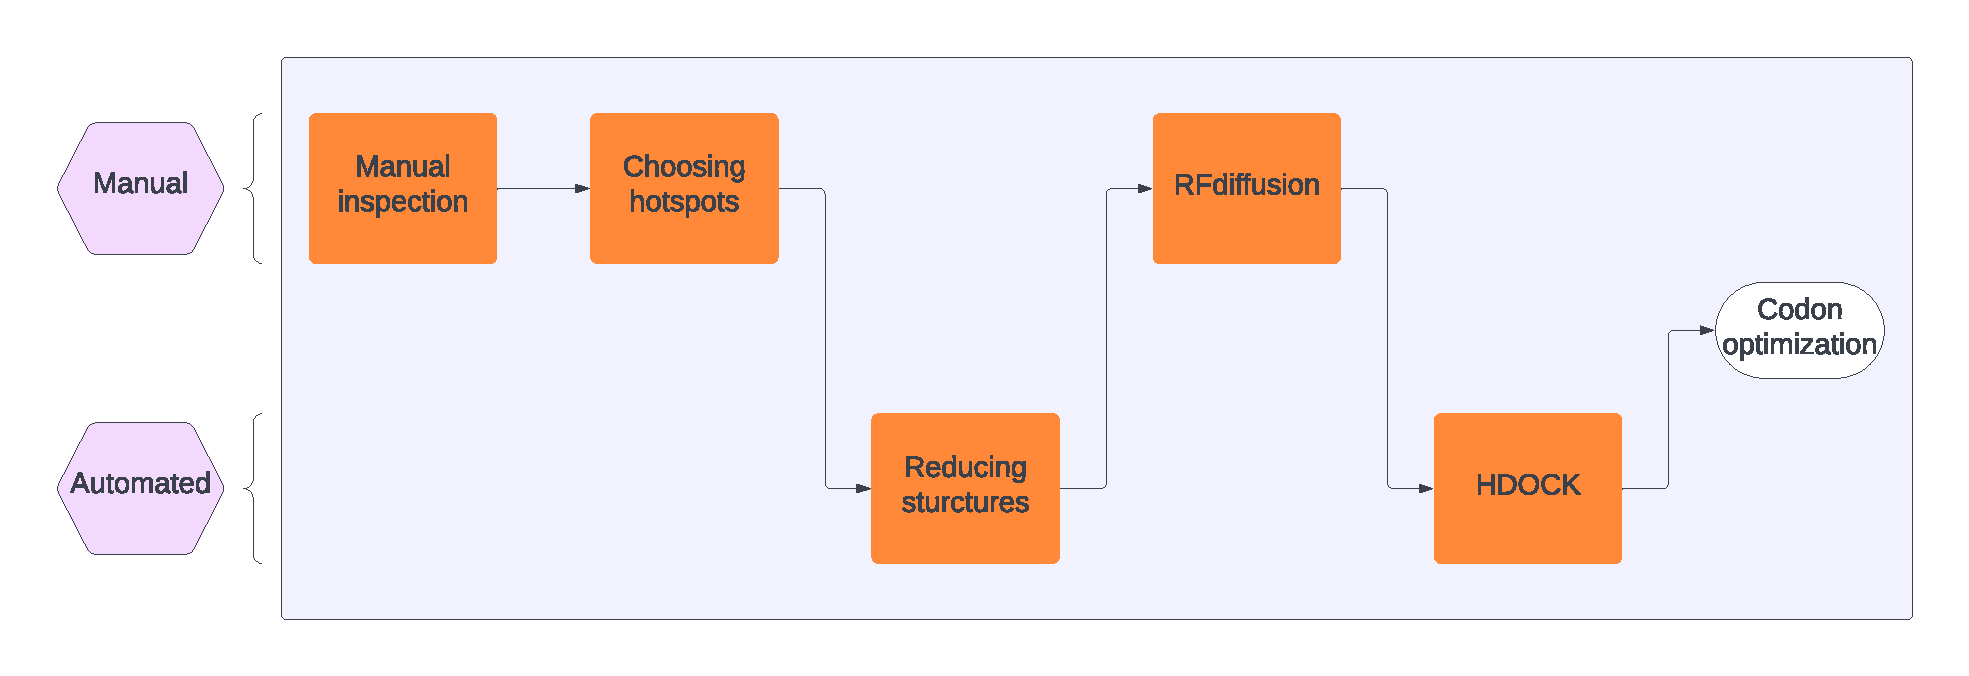
\includegraphics[width=\textwidth]{Figures/iGEM_project_general_organization_graph.pdf}
    \caption{General organization graph of the iGEM project.}
\end{figure}

\subsection{Target Protein Inspection and Hotspot Selection}

Commencing with the delineation of a hotspot, we define it as a specific residue (amino acid) on the target protein that we aim for the designed binders to effectively bind to. Despite the potential ambiguity of this term, our adoption of RFdiffusion's terminology guides our terminology usage.

Our strategy for selecting potential binding sites involved both manual inspection and the identification of hotspots based on specific rules of thumb. We developed these rules of thumb through a combination of manual exploration and adjustments based on RFdiffusion guidance.

Alexis Courbet, a former member of the Baker lab, significantly contributed to shaping our guiding principles for binder design. Leveraging his expertise, we established a set of criteria to guide our manual inspection process, focusing on identifying residues that align with the following:

\begin{itemize}
\item Target regions exhibiting high solvent accessibility.
\item Regions characterized by noticeable hydrophobic patches.
\item Grooves within the target structure.
\end{itemize}


In accordance with the established criteria, we opted for Human Papillomavirus (HPV) as one of our targets due to its nature as a naked virus (non-enveloped) /cite{morshed2014human}. At the initial stages of our exploration with RFdiffusion, the potential interference of glycoproteins with our study was uncertain. To address safety concerns, our strategy involved expressing the proteins in an alternative vector rather than utilizing the actual virus.

The selection of Bacteriophage T4 was motivated by its availability in our laboratory and the associated safety considerations. Unlike HPV, using the virus in its native form was feasible and, with HPV proteins, presented a robust proof of concept for our study.

To select hotspots, ChimeraX functionalities such as "hydrophobic" and "electrostatic" were utilized, generating color-coded surfaces to visualize hydrophobic to hydrophilic and negative to positive surfaces on the protein structure. Ultimately, ChimeraX proved to be a valuable open-source tool for implementing our guidelines, enabling the effective identification of essential hotspots.

\subsection{Running RFdiffusion}

Due to the substantial size of capsids, which are intricate protein assemblies, computational limitations necessitated the pruning of structures around identified hotspots to prevent out-of-memory errors. To streamline this process and minimize potential errors and biases introduced by manual steps, a custom code was developed using the BioPython library. The code automates the reduction of structure based on predefined criteria, ensuring a more efficient and standardized approach.

These reduced sturcte are then manually used as input for RFdiffusion. To comply with legal restrictions, local code execution or connecting a local session to Google Colab is prohibited, as outlined in the \href{https://research.google.com/colaboratory/faq.html#disallowed-activities}{Google Colab disallowed activities}. Therefore, the results of the structure-reducing scripts were manually uploaded to the Google Colab Virtual Machine. If access to a robust local GPU were available, further automation of the entire process, after choosing the hotspots. 

\subsection{HDOCK: an orthogonal validation approach}

After completing the previous steps, the number of generated sequences reached the order of thousands. However, the practical constraints of our team's budget made it unfeasible to test all these sequences experimentally. To prioritize potential designs and narrow down the candidates for experimental validation, we sought an orthogonal approach for assessment.

Through extensive research, we chose to employ HDOCK, an \emph{in-silico} binding tool known for its consistent performance in the CASP-CAPRI \cite{casp-capri} competition over the years. HDOCK utilizes a fast rigid-body docking algorithm, which can be parallelized on a server to enhance throughput, enabling the scanning of numerous potential designs within a reasonable timeframe.

We applied an \emph{in-silico} filtration steps using a customized code that I develpoed to parallelize the process and get all the needed statistics. Only the sequences deemed most likely to exhibit binding were retained for further experimental validation.

\subsection{To delete}

\subsubsection{Task description}
(1-2 pages with figures if relevant): (Methods is a section valid for any internship, not only research-oriented, experimental or theoretical. You did something according to a method, which is what you should understand and present here.)
Present in detail the tools, techniques and methods you have used and why (giving a list of library's or equipment's name is not a presentation). 
Describe the scientific and/ or technical background with clear explanations, references, equations and/ or schematics or pictures. 

\subsubsection{Key points}

\begin{itemize}
    \item This section should be prttey consise in terms of word, but 
    full of screenshots about the used tools.
    \item Here I can totally start pointing out to the graph where I 
    have the entire pipline.
    \item Talk about RFdiffusion. How it works, talk about Sergey's 
    Google Colab adaptation.
    \item Talk BRIEFLY about ChimeraX. and how you used it to find the 
    targets of interest.
    \item Talk about different docking tools. Also the two contests for 
    docking.
    \item Mention how HDOCK scored pretty good in these ones, and also 
    how is it free to download.
    \item Talk about parrallel computing, and talk about parrallel 
    computing using Python. and how you used this to further speed up 
    the process of docking.
\end{itemize}


\section{Results}

After manually inspecting the following proteins:

\begin{itemize}
    \item HPV major capsid protein (PDBID 7kzf)
    \item Bacteriophage T4 capsid (PDBID 7vs5)
    \item Bacteriophage T4 Long-Tail (PDBID 2xgf)
    \item GFP protein (PDBID 5b61)
\end{itemize}

I picked around 50 different sets of hotspots. Each set contains 2 to 4 hotspots. \textcolor{red}{Point to the table}. Each set of hotsopt will be called a "run" from now on.

Each run can produce $S*Q$ sequences, where $S$ is the number of structure backbones that RFdiffusion algorithm should predict in the first step, and $Q$ is the number of sequences generated per structure backbone using the NPMM step.
generate

\subsection{To delete}

\subsubsection{Task description}
(2-3 pages with figures):
Precisely describe the results of your work with clear explanations of 
the analysis, schematics and figures.
Describe what worked, what didn't and why.

\subsubsection{Key points}


\begin{itemize}
    \item Here there's two catches:
    \begin{itemize}
        \item I have generated data for two targets but only one was 
        tested.
        \item I have really results that can be described totally in 
        few sentecs.
    \end{itemize}
    \item Talk about how many structures you generated.
    \item Talk about the tendecy of short ones to have repeated 
    sequences. Come up with some metrics to measure this.
    \item just come up with some metrics to fill the page.
    \item Talk about the docking results. How good, bad they were.
    \item Talk about the i\_PAE score, why you didn't use it from the 
    begining?
    \item Show some nice graphs about the docking results. with color 
    coding everhting, and the ones picked.
    \item Ask Louis, Momo, and/or Avi for help on the wet lab part (it 
    should be a small sub-section).
    \item There's a side hustles, a result should be visually 
    appealing. So talk how I used ChimeraX to generate some cool 
    animations. Talk about other new tools in development like the one 
    I found during a lab meeting at Jussieu (I don't if the name is 
    correct). 
\end{itemize}

\subsubsection{Text}

Lorem ipsum dolor sit amet, consectetur adipiscing elit.

% Discussion
\section{Discussion}

\subsection{To delete}

\subsubsection{Task description}
(1 page): 
Review findings.
Discuss outcomes.
Do your results make sense ? 
Evaluate them
Do they provide elements towards solving your problem ? Which ones ?
Do they open up new questions (scientific or technical).

\subsubsection{Key points}

Lorem ipsum dolor sit amet, consectetur adipiscing elit.

\subsubsection{Text}

Lorem ipsum dolor sit amet, consectetur adipiscing elit.

% Conclusion
\section{Conclusion}

\subsection{To delete}

\subsubsection{Task description}
($\frac{1}{2}$ to 1 page maximum):
Conclude regarding the missions and tasks you were given and the 
results you obtained . Mention if they will be used by your team. 
What are the limitations of your results ?
What are the future directions (questions, implementation…) ? 

\subsubsection{Key points}

Lorem ipsum dolor sit amet, consectetur adipiscing elit.

\subsubsection{Text}

Lorem ipsum dolor sit amet, consectetur adipiscing elit.

% Acknowledgments
\section{Acknowledgments}

\subsection{To delete}

\subsubsection{Task description}
Also conclude regarding your work at the institution, your integration 
to the team, what you brought, what you have learned, what you need to 
improve.

\subsubsection{Key points}

\begin{itemize}
    \item My colleages.
    \item Minc lab.
    \item two people whom I emailed for help.
    \item Others.
\end{itemize}

\subsubsection{Text}

Lorem ipsum dolor sit amet, consectetur adipiscing elit.

% References
\printbibliography

% Annexes
\section{Annexes}

\subsection{To delete}

\subsubsection{Task description}

(3 pages maximum, if needed)
Add experimental details, code, algorithms, figures, pictures and any 
additional information we need to understand your work. Links welcome.
Organize them freely but clearly.

\subsubsection{Key points}

Lorem ipsum dolor sit amet, consectetur adipiscing elit.

\subsubsection{Text}

Lorem ipsum dolor sit amet, consectetur adipiscing elit.

\section{What else?}

Data. 
Why do you need them ? How and when were they collected, stored, accessed, selected and sorted ? Describe the data you used (information they contain, length, format, database,...) . Describe their limitations. Precise the legal and ethical context.

Implementation. 
Describe the operation pipelines with clear explanations and schematics. What is your detailed contribution here (experiment, code, algorithm, operation…) ? What have you implemented (and modified) ? How have you implemented it ? 


\end{document}